
\section{Results}
\begin{figure*}[htbp]
	\centering
	\subfigure[espresso]{
		\label{fig_10_1}
		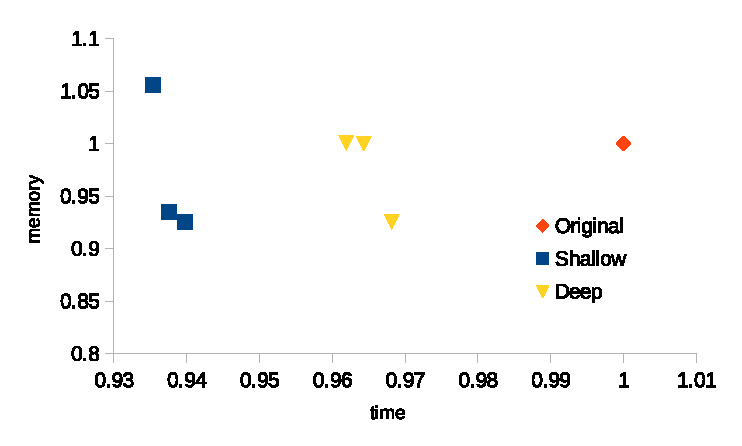
\includegraphics[width=0.4\textwidth]{fig10}
	}
	\subfigure[space]{
		\label{fig_10_2}
		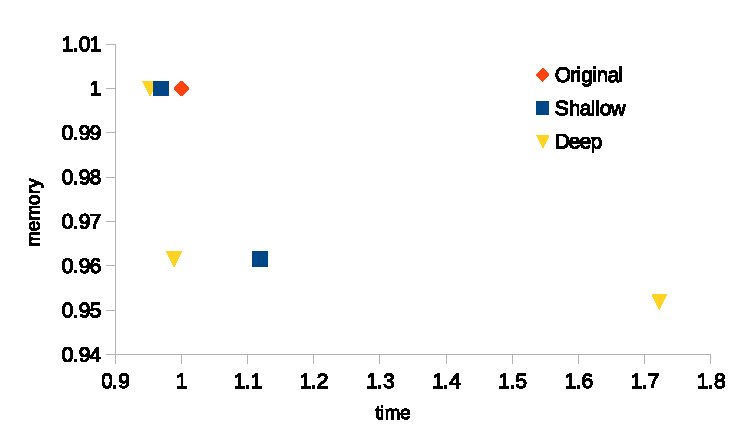
\includegraphics[width=0.4\textwidth]{fig12}
	}
	\subfigure[cfrac]{
		\label{fig_10_3}
		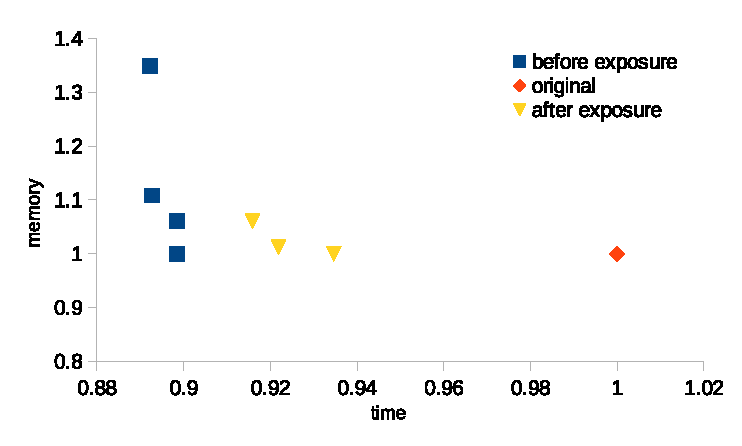
\includegraphics[width=0.4\textwidth]{fig13}
	}
	\subfigure[gawk]{
		\label{fig_10_4}
		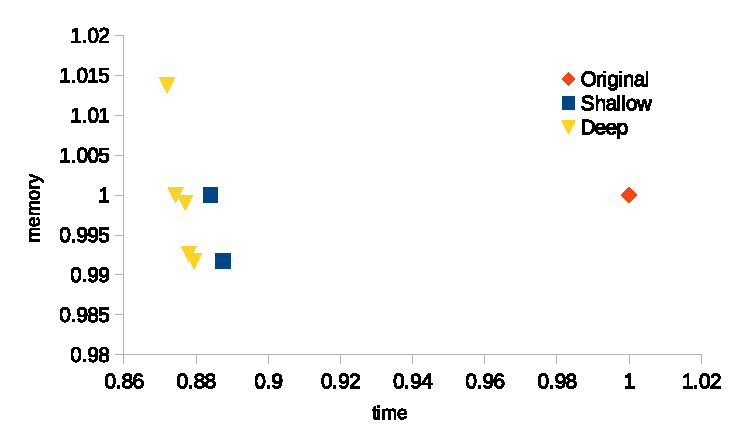
\includegraphics[width=0.4\textwidth]{fig14}
	}
	\caption{Pareto-best individuals for each application, ``before exposure'' points are abtained without tuning TOP\_FOOT\_SIZE and ``after exposure'' points with TOP\_FOOT\_SIZE tuned. Less memory and time is better.}\label{fig_10}
\end{figure*}


\subsection{Shallow Parameter Tuning Improvement}

**How much did we improve comparing to default?

**How much did we improve comparing to random?

**What is the implication?


\subsection{Deep Parameter Tuning Improvement}


**How much more did we improve comparing to default?

**How much more did we improve comparing to random?

**How much more did we improve comparing to random?

**What is the implication?


The result for each application is depict in Figure \ref{fig_10}. All the time and memory consumptions shown in the figures are normalized to the consumption of running the corresponding application with the original \emph{dlmalloc}. The figures show that by tuning these parameters, we could achieve up to 11\% reduction on the time consumption (gawk, Figure \ref{fig_10_4}), and 7.5\% reduction on the memory usage (espresso, Figure \ref{fig_10_1}). The square points in each graph are the non-dominated individuals with parameter TOP\_FOOT\_SIZE intact, meaning in these individuals only the first 9 parameters are adjusted to the application. Without the parameter TOP\_FOOT\_SIZE tuned, we can get comparable but slightly worse results. After the parameter TOP\_FOOT\_SIZE is exposed and considered in the search space, clearly the Pareto front is widened and a little better performance is achieved.
\begin{table*}[hbtp]
\centering
\caption{Best individuals for each application}
\label{tab_2}
\resizebox{0.8\textwidth}{!}{
\begin{tabular}{c|c|c|c|c}
\hline
\textbf{\emph{espresso}} & time(s) & normalized time & memory(kB) & normalized memory \\
\hline
original & 4.773 & 100\% & 5152 & 100\% \\
\hline
most-time-saving before exposure & 4.667 & 97.8\% & 5440 & 105.6\% \\
\hline
most-time-saving after exposure & 4.638 & 97.2\% & 6272 & 121.7\% \\
\hline
most-memory-saving before exposure & 4.689 & 98.2\% & 4768 & 92.5\% \\
\hline
most-memory-saving after exposure & 4.654 & 97.5\% & 4768 & 92.5\% \\
\hline
\hline
\textbf{\emph{space}} & time(ms) & normalized time & memory(kB) & normalized memory \\
\hline
original & 19.3 & 100\% & 416 & 100\% \\
\hline
most-time-saving before exposure & 18.7 & 96.9\% & 416 & 100\% \\
\hline
most-time-saving after exposure & 18.0 & 93.2\% & 416 & 100\% \\
\hline
most-memory-saving before exposure & 21.6 & 111.8\% & 400 & 96.2\% \\
\hline
most-memory-saving after exposure & 39.9 & 206.3\% & 396 & 95.2\% \\
\hline
\hline
\textbf{\emph{cfrac}} & time(s) & normalized time & memory(kB) & normalized memory \\
\hline
original & 1.071 & 100\% & 332 & 100\% \\
\hline
most-time-saving before exposure & 0.956 & 89.2\% & 448 & 134.9\% \\
\hline
most-time-saving after exposure & 0.981 & 91.6\% & 352 & 106\% \\
\hline
most-memory-saving before exposure & 0.962 & 89.8\% & 332 & 100\% \\
\hline
most-memory-saving after exposure & 1.001 & 93.5\% & 332 & 100\% \\
\hline
\hline
\textbf{\emph{gawk}} & time(s) & normalized time & memory(kB) & normalized memory \\
\hline
original & 2.711 & 100\% & 4356 & 100\% \\
\hline
most-time-saving before exposure & 2.396 & 88.4\% & 4356 & 100\% \\
\hline
most-time-saving after exposure & 2.389 & 88.1\% & 4320 & 99.2\% \\
\hline
most-memory-saving before exposure & 2.406 & 88.8\% & 4320 & 99.2\% \\
\hline
most-memory-saving after exposure & 2.389 & 88.1\% & 4320 & 99.2\% \\
\hline
\end{tabular}}
\end{table*}

\subsection{Understanding the Exposed Parameters}

** Add a table of all exposed parameters and add a paragraph to brief expalin them.

The most time-saving and memory-saving individuals before or after exposing TOP\_FOOT\_SIZE are list in Table \ref{tab_2}. The interesting thing is, by finding the optimal values for these parameters, we can improve both memory and time at the same time. For instance, the most memory-saving individual for \emph{space} after TOP\_FOOT\_SIZE exposed costs 97.5\% of the original time cost while using only 92.5\% of the memory used by the original allocator. However, some of these application can not be improved by our approach in terms of time or memory. No improvement in memory consumption has been found in \emph{cfrac}, and the time saved for \emph{space} is not significant compared to the noise introduced in this experiment. Another interesting thing we learned in this study is, for different applications, the optimal values for those parameters are quite different. In another word, the optimal values for one application don't guarantee to improve other applications.


(**explain why TOP\_FOOT\_SIZE can influence dlmalloc's behavior)
\textbf{TOP\_FOOT\_SIZE} controls how many extra bytes should be included in the top chunk while the allocator extends the top chunk. It influences how much more memory than actually needed \emph{dlmalloc} should keep to buffer allocation and deallocation. Bigger TOP\_FOOT\_SIZE tends to cost more memory but possibly saves some costly system allocation and deallocation. The optimal value could vary across applications. Originally it is a constant determined by some macros and system related parameters. We now make it to a tunable parameter and expose it to users so that it can be changed at compilation like other configurations.
